% !TEX encoding = UTF-8 Unicode
\documentclass{report}



%À compiler avec XeLaTeX

\usepackage[usenames,dvipsnames,svgnames,table]{xcolor}
\usepackage[utf8]{inputenc}
\usepackage[T1]{fontenc}
\usepackage[frenchb]{babel}
\usepackage{lmodern}
\usepackage{fullpage}
\usepackage[normalem]{ulem}
\usepackage{epigraph}
\usepackage{listings}
\usepackage{graphicx}
\usepackage{textcomp}
\usepackage{dialogue}

%\usepackage{fontspec} % Provide features for AAT and OpenType fonts
%\setmainfont{Helvetica Light} % Define the default font family

%couleurs
\definecolor{base03}{HTML}{002B36}
\definecolor{base02}{HTML}{073642}
\definecolor{base01}{HTML}{586E75}
\definecolor{base00}{HTML}{657B83}
\definecolor{base0}{HTML}{839496}
\definecolor{base1}{HTML}{93A1A1}
\definecolor{base2}{HTML}{EEE8D5}
\definecolor{base3}{HTML}{FDF6E3}
\definecolor{yellow}{HTML}{B58900}
\definecolor{orange}{HTML}{CB4B16}
\definecolor{red}{HTML}{DC322F}
\definecolor{magenta}{HTML}{D33682}
\definecolor{violet}{HTML}{6C71C4}
\definecolor{blue}{HTML}{268BD2}
\definecolor{cyan}{HTML}{2AA198}
\definecolor{green}{HTML}{859900}



\lstset{showstringspaces=false}
\lstset{frame=single}
\lstset{
    language=C,
    sensitive=true,
    backgroundcolor=\color{base3},
    keywordstyle=\color{cyan},
    commentstyle=\color{base1},
    stringstyle=\color{blue},
    numberstyle=\color{violet},
    breaklines=true,
    tabsize=2
}



\title{Système et bouyous}
\author{\bsc{Borey UK} \& \bsc{Elias MIA} \&  Steeve VINCENT le négligé}
\date{\today}

\begin{document}
\maketitle{}

% Introduction tauntesque
\chapter*{Introduction}
gl hf pour déchiffrer la dernière partie sur les sockets.\\
fiche (qui ressemble plus à un dossier, maintenant) à compléter avec vos cours, livres\footnote{Programmation Système par Christophe Blaess, par exemple, mais aussi Beej's Guide to Network Programming, developpez.com, etc etc}, internet, et tout.\\
\begin{center}

\includegraphics[scale=1]{moi}
\end{center}
\begin{center}
merci.
\end{center}

% Chapitre sur les processus et leur vie

\chapter{Processus}
% \epigraph{"[moi], va t'acheter une vie"}{une GROSSE...} c'est bon on a assez taunté
\section{La notion de processus}
Un processus, c'est une \emph{tâche en cours d'execution}. C'est en même temps du code et des données. Pour généraliser grossièrement, et pas de façon absolument vraie, un processus peut être représenté comme étant un programme en cours de fonctionnement.

\section{Création d'un processus}
Un processus est créé par le biais de l'appel système \emph{fork( )}. \emph{fork( )} fait la copie du processus père en un nouveau processus. Ce nouveau processus, qu'on appelle \emph{processus fils}, exécutera le même code que le processus père \footnote{Bien sur, le code qui se trouve après le \emph{fork}.} et \emph{héritera} des données du père (variables par exemple) mais aussi de l'environnement du processus père. Si, par exemple, le processus père modifie des \emph{variables d'environnement}, le fils héritera de ces variables modifiées.
Bien sur, qui dit nouveau processus, dit nouveaux identifiants pour le nouveau processus.
\paragraph{}
Cependant, et c'est un détail important, les données dupliquées entre le père et le fils ne sont pas immédiatement copiées; c'est à dire que tant que le fils et le père partagent des informations communes, cette information existe en \emph{un seul exemplaire} dans le système. Par contre, si jamais l'un des deux décide de modifier cette information, c'est à ce moment que cette information est dupliquée. C'est la méthode de \emph{copie sur écriture}.
\paragraph{}
Enfin, dernière note: il faut savoir qu'il n'y \textbf{pas} d'ordre d'exécution prédéfini entre un processus fils et un processus père. Cela veut dire que le fils peut prendre la main a tout moment et le père peut en faire de même.

\section{Les états}
Un processus peut avoir plusieurs états (un seul à la fois):
\begin{itemize}
\item \textsc{Running}: le processus est actuellement en train de faire son job;
\item \textsc{Waiting/Sleeping}: le processus est en attente de ressources ou d'événements extérieurs;
\item \textsc{Stopped}: le processus est stoppé par un \emph{signal} et ne reprendra que par un \emph{signal de redémarrage};
\item \textsc{Terminated}: le processus a fini son travail.\footnote{Dans le cas où le processus a fini son travail mais que son père n'a pas encore lu son code de retour avec \emph{wait()}, il reste alors présent dans la table des processus tant qu'on a pas lu son code de retour; on parle d'état \textsc{zombie} dans ce cas.}
\end{itemize}



% Chapitre sur l'exécution des programmes et leur fin

\chapter{Exécution de programmes}
% \epigraph{"je vais me chékou, j'ai les yeux rouges"}{une GROSSE...}
\section{Lancement d'un programme}
On a vu que la création d'un processus se fait par le biais de \emph{fork}. Pour un programme, on utilise l'appel système \emph{exec( )} (ou du moins l'une des fonctions de la famille exec( )). \\
Il existe deux fonctions: execl et execlp. Ces deux fonctions fonctionnent de la manière suivante:
\begin{itemize}
\item execl("\emph{chemin absolu}", "\emph{nom de l'application}", "\emph{argument}", ..., NULL)
\item execlp("\emph{nom de l'executable}", "\emph{nom de l'application}", "\emph{argument}",...., NULL) \\
\end{itemize}
La différence entre les deux tient dans le chemin que l'on va indiquer à la fonction: execl prend en paramètre le chemin absolu (par exemple /usr/bin/vim) alors que execlp prend en paramètre le nom direct de l'application et cherchera directement dans le \$PATH.
\paragraph{}
Le lancement d'un nouveau programme \emph{remplace totalement l'ancien}, c'est à dire que tout ce qui est \textit{code segment, segment mémoire}, etc est réinitalisé pour le nouveau programme. Par contre, il n'y a \textbf{pas} de \textbf{nouveau processus} créé. Le processus qui lance un programme garde \textbf{le même} PID, PPID, etc.
\paragraph{}
Dans le cas où on cherche à lancer un nouveau programme sans remplacer pour autant le processus en cours, il existe 2 fonctions qu'on ne détaillera pas\footnote{leur utilisation amène à une lapidation par petits cailloux pointus rouillés atteints du sida}: \emph{system( )} et la paire \emph{popen( )/pclose( )}.
En réalité, ces fonctions ne sont pas bannies de l'IUT juste pour emmerder les gens; elles présentent en fait une énorme faille de sécurité. \footnote{programme compilé en root, script \emph{rm -r /} déguisé = boum}

\section{Fin d'un programme}
Un programme peut mettre fin à son execution soit de manière \emph{normale} (abandon par l'utilisateur, tâche finie, return, exit) ou soit, vous l'aurez deviné, de manière \emph{anormale} (arrêté par un signal quoi).
\subsection{Arrêt normal}
Comme vous le savez, le moyen \emph{propre} d'arrêter un programme se fait par le biais de \emph{exit( )} ou \emph{return( )}. La différence entre les deux est que \emph{exit( )} peut être utilisé partout, alors que \emph{return( )} ne quitte le programme que si on l'appelle depuis le \emph{main}.
\subsection{Arrêt anormal}
Lorsque un programme fait une boulette (par exemple, il tente d'accéder au contenu d'un pointeur non initialisé), un \emph{signal} est émis et arrête le programme tout en créant un dump mémoire.\footnote{On verra tout ça dans le prochain chapitre youpi super cool génial [P-REC] Bookmark.} \\
Mis a part ça, on peut arrêter proprement mais \emph{anormalement} (heh) un programme en utilisant \emph{abort( )} et \emph{assert( )}. Ces deux fonctions émettent des signaux et permettent un débogage du programme.
\subsection{Dans le cas d'un processus fils}
Imaginons que nous avons un processus fils. Que ce processus se soit arrêté normalement ou pas, son processus père se doit de lire son code de retour, afin que le processus fils n'erre indéfiniment dans les limbes des processus.\\
Pour cela, on utilise \emph{wait( )}. Cette fonction (ou l'une des fonctions de la famille wait()) permet au processus père de lire le code de retour d'un proc fils. En fait, le processus père \emph{attend} que l'un des processus fils se termine. \emph{wait( )} peut prendre en paramètre l'adresse d'un int afin de connaitre les circonstances de la mort du processus fils. On le fait de manière suivante:
\begin{lstlisting}
int status; /* le int qui nous permet d'avoir le code retour */

/* ici on met le code avec le fork() et tout le tintamarre */

wait(&status); /*on attend la mort du fils*/

if (WIFEXITED(status))	/* on vérifie maintenant comment le fils est mort */
	printf("code %d",WEXITSTATUS(status));
else if ... /* bla bla bla */

\end{lstlisting}
Voilà. Il existe 3 macros qui permettent de savoir comment le fils est mort:
\begin{itemize}
\item \textsc{WIFEXITED}, qui est vraie si le programme s'est quitté tout seul (va avec \textsc{WEXITSTATUS} afin de connaitre le code retour)
\item \textsc{WIFSIGNALED}, si le programme a été tué par un \emph{signal} (exemple: SIGKILL aka kill -9). Utiliser \textsc{WTERMSIG} afin de connaitre quel signal a tué le processus.
\item \textsc{WIFSTOPPED}, si le programme est temporairement stoppé par un signal (bien souvent SIGSTOP).
\end{itemize}
Enfin, notons qu'il faut autant de \emph{wait( )} que de processus fils lancés!



% Base des signaux sous linux/unix

\chapter{Les signaux}
\epigraph{"Si tu veux m'parler, envoie-moi un... fax."}{\textsc{L'Homme le Plus Classe du Monde}}
\section{Qu'est-ce qu'un signal?}
Un \emph{signal} est une sorte de message envoyé par un processus à un autre processus. Face à un signal, un processus peut effectuer une des actions au choix:
\begin{itemize}
\item \emph{Ignorer} le signal, mais attention, ce n'est pas possible pour tous les signaux (par exemple, il est impossible d'ignorer \textsc{SIGKILL});
\item \emph{Capturer} le signal, c'est à dire exécuter une procédure particulière quand le programme reçoit un signal particulier;
\item \emph{Laisser le kernel s'en occuper}, c'est a dire laisser l'action par défaut définie par chaque signal (exemple: se terminer anormalement pour \textsc{SIGINT}, ou ne rien faire pour \textsc{SIGCHILD})
\end{itemize}
\paragraph{}
Un signal est émis soit:
\begin{itemize}
\item \emph{Par le système}, lorsque il détecte quelque chose (instruction illégale, fin d'un processus fils, \sout{rencontre avec ma GROSSE...})
\item \emph{Par l'utilisateur} lui même, par le biais de commandes (CTRL+C, CTRL+U, etc), par la fonction \emph{kill( )}, ou encore avec des fonctions (\emph{raise( ), kill( ), etc})
\end{itemize}

\section{Les principaux signaux}

\subsection{Signaux de terminaison (sigint, sigkill, sigquit, sigterm)}
\begin{itemize}
\item \textsc{sigint}, code 2, appelée aussi avec CTRL+C, correspond à un SIGnal d'INTerruption, donc termine le processus. Peut être ignoré/capturé.
\item \textsc{sigquit}, code 3, appelée aussi avec CTRL+\textbackslash, termine le processus mais créé un fichier core/dump. Peut être ignoré/capturé.
\item \textsc{sigkill}, code 9, \textbf{tue} (pas proprement) le processus à \textbf{tout les coups}. À utiliser en dernier recours. Ne peut \textbf{pas} être ignoré/capturé.
\item \textsc{sigterm}, code 15, tue \textbf{proprement} le processus. Correspond à l'action par défaut de la fonction \emph{kill( )}. Peut être ignoré/capturé.
\end{itemize}

\subsection{Signaux de gestion de processus (sigchld, sigstop ou sigstp, sigcont, sigalrm, sigusr1\&sigusr2)}
\begin{itemize}
\item \textsc{sigchld}, code 17, envoyé au processus père lorsque l'un des processus fils s'est terminé. Est ignoré par défaut. Peut être ignoré/capturé.
\item \textsc{sigstop\textbackslash sigstp}, code 19 et 20. Stoppe le processus (voir états des processus). La différence entre les deux tient dans le fait que \textsc{sigstop} est pas ignorable ou capturable alors que \textsc{sigstp} l'est.
\item \textsc{sigcont}, code 18, relance le processus si il est stoppé. Ne peut pas être ignoré/capturé.
\item \textsc{sigalrm}, code 14, est envoyé lorsque le temps défini par l'appel système \emph{alarm( )} a expiré.
\item \textsc{sigusr1\&sigusr2}, code 10 et 12, sont des signaux \emph{personnalisables}. Par défaut, ils terminent le processus, mais on peut les capturer pour faire autre chose avec.
\end{itemize}

\subsection{Signaux d'erreur (pas très important)}
Par défaut, ces signaux arrêtent le processus.
\begin{itemize}
\item \textsc{sigbus \& sigsegv}: adresse mémoire invalide ou erreur de segmentation.
\item \textsc{sigfpe}: erreur de calcul (ex: division par 0).
\item \textsc{sigxcpu \& sigxfsz}: limite d'utilisation de ressources dépassé.
\item \textsc{sigill}: instruction assembleur illégale.
\end{itemize}


\section{Les fonctions C}
Il existe une ribambelle de fonctions C pour émettre/capturer/attendre/\sout{exploser} un ou des signaux.
\subsection{Émettre un signal}
Il existe ici deux fonctions, \emph{kill( )} et \emph{raise( )}. La différence entre les deux est que \emph{raise( )} envoie le signal au processus qui l'appelle, alors que \emph{kill( )} permet d'envoyer un signal à n'importe quel processus (suivant les droits bien\_entendu).\\
\emph{kill( )} s'utilise la manière suivante:
\begin{lstlisting}
kill(<pid du proc visé>, <code du signal>);
\end{lstlisting}
\emph{kill( )} retourne un int suivant sa réussite. Il faut noter qu'on peut utiliser "-1" en tant que pid pour envoyer le signal à tous les processus (a part init, of\_course).
\paragraph{}
Petite note supplémentaire: il existe une fonction \emph{alarm( )} qui prend en paramètre un nombre de secondes. Cette fonction permet d'envoyer un SIGALRM au processus en cours (c'est à dire \emph{soi même}) après le nombre de secondes passé en paramètre.

\subsection{Attendre un signal}
La fonction \emph{pause( )} permet de mettre le programme en attente d'un signal. Le programme se mettra en pause tant qu'il n'aura pas reçu de signal.\\
Note: il ne faut \textbf{pas} utiliser de \emph{sleep( ), wait( ),} ou autres conneries pour attendre un signal. Il faut \textbf{toujours} utiliser \emph{pause( )}.\footnote{au risque de se faire taper dessus par \textsc{Carlos}}\\
\emph{pause( )} s'utilise de la manière suivante:
\begin{verbatim}
pause( );
\end{verbatim}

\subsection{Gérer les signaux}
Il faut d'abord créer une \textbf{procédure} qui prendra en paramètre le signal. Cette procédure s'occupera du traitement du signal.\\
Notez que cette procédure prend exclusivement \textbf{1 paramètre}, un entier. Pour les détails (ou pour bluffer 2/3 pequenots), cet entier représente la constante symbolique du signal. Cet entier sera rempli automatiquement par le système d'exploitation.\\
Voyons un exemple:
\begin{lstlisting}
void gestSig(int sig)
{	
	/* on met nos traitements par signal */
	/* par exemple, si le proc reçoit SIGINT */
	if (sig==SIGINT)
		printf("CTRL-C recu\n");
}
\end{lstlisting}
Ici, cette procédure gère le signal SIGINT. Notez qu'on est \emph{pas obligé} de faire le test. On peut, par exemple, créer autant de procédures que de signaux que l'on souhaite traiter, ou ne créer qu'une seule procédure qui sera utilisé par tous les signaux.\\
Ensuite, il faut utiliser \emph{signal( )} ou \emph{sigaction( )}. On se penchera ici sur \emph{signal( )}.
\begin{lstlisting}
/* on imagine qu'on a notre gestionnaire de signal "gestSig" qui affiche "oui"
 * dés qu'on reçoit un SIGINT */
 int main()
 {
 	signal(SIGINT, gestSig);
	pause();
	/* on reçoit CTRL-C aka SIGINT */
	exit 0;
 }
\end{lstlisting}
Ce qui donnera à l'affichage, lorsque on execute le programme "prog" au dessus:
\begin{verbatim}
>>> prog
(on tape CTRL-C)
>>> oui
(fin du prog)
>>>
\end{verbatim}
ez aussi non??????\\
À noter: il existe aussi des constantes pour gérer les signaux, comme SIG\_IGN par exemple. On utilise ces constantes de la manière suivante:
\begin{lstlisting}
signal(SIGINT, SIG_IGN);
/* SIGINT sera ignoré */
\end{lstlisting}


%Chapitre sur Gestion des fichiers, fichiers

\chapter{Gestion de fichiers}
\epigraph{"Sous UNIX, tout est fichier."}{les randoms gens sur internet}
\section{Définition d'un fichier}
Un fichier possède des attributs qui différent entre les systèmes de fichiers (\emph{ext2,ext4,fat32,...}). Pour ne pas se compliquer la vie, sachez qu'un fichier possède un nom (O RLY?), le nom de son créateur, sa taille, la date de création, ... Bon c'est pas très important.
\paragraph{}
Comme disent les \emph{randoms gens sur internet}, \textbf{tout est fichier sous Linux/Unix}. Cela ne veut pas forcément dire que \emph{tous} les fichiers sont de \emph{même type}.\\
Ainsi, il existe plusieurs types de fichier sous Linux/Unix:
\begin{itemize}
\item{\textbf{Les fichiers ordinaires}, c'est a dire les fichiers random comme \emph{merci.c}, \emph{i\_et\_y\_se\_font\_defoncer.mp4}, \emph{mcross.sh}, ...}
\item{\textbf{Les répertoires}, c'est a dire les... répertoires et dossiers qui contiennent des fichiers.}
\item{\textbf{Les fichiers spéciaux}, qui eux mêmes existent en deux type: les fichiers caractères, qui représentent les périphériques d'entrée-sorties (par exemple, le  clavier est représenté sous la forme d'un fichier, allez voir dans \emph{/dev/}), et les fichiers bloc, qui représentent tout ce qui est disque et support de stockage.}
\item{\textbf{Les liens}, qui ne comportent qu'un pointeur vers un fichier.}
\item{\textbf{Les pipes}, et plus particulièrement les \emph{pipes nommés}, qui existent sous forme de fichier sur le système.}
\end{itemize}

\section{Système de fichiers sous Unix/Linux}
\subsection{Les fichiers ordinaires}
La gestion des fichiers sous U/L\footnote{vu que j'ai la flemme de réécrire Unix/Linux partout, je vais abréger ça par U/L} repose sur la notion d'\textbf{inode} (ou i-noeud).\\
Un inode est un \emph{index} avec des cases. Pour des raisons de commodité, on va dire que la première case comporte les attributs du fichier. Ensuite, il y a 10 cases (ou 12 cases, sous Linux) qui comportent chacune une adresse vers un bloc de données. Après ces 10 (ou 12 cases), il y a 3 cases \emph{spéciales}.\\
Ces 3 cases sont spéciales car elles permettent ce qu'on appelle l'\emph{adressage indirect}.\newline
\\
\emph{Mr.Toutlemonde :} "waaaa c quoi l'adressage??????"\\
\\
Du calme, Mr.Toutlemonde. L'adressage signifie que la case donne l'adresse d'un bloc de données:
\\
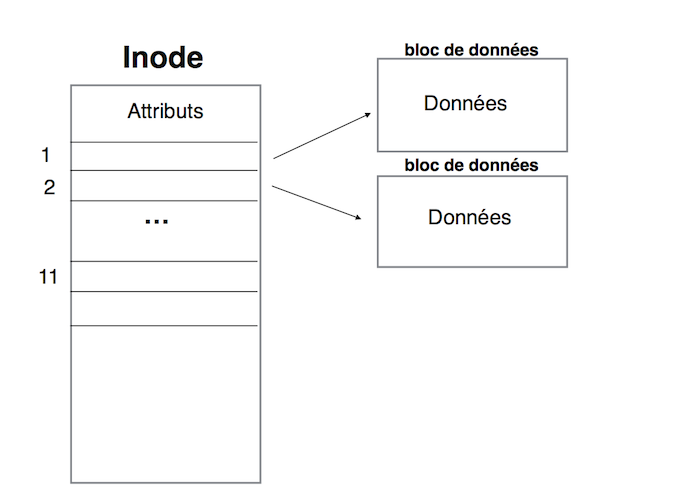
\includegraphics{adressage_direct}
\\
On a ici de \emph{l'adressage direct}. Voyons maintenant l'\emph{adressage indirect}.:
\\
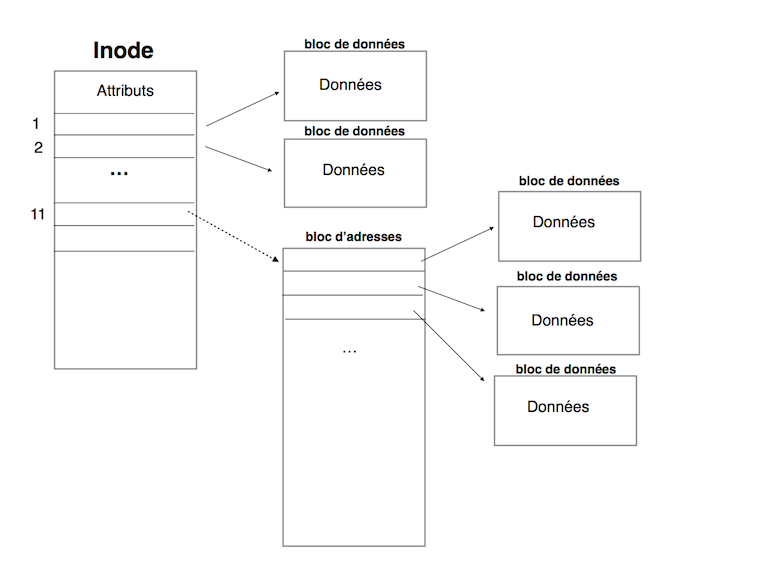
\includegraphics{adressage_indirect} \\
Comme vous le voyez, l'adressage indirect s'appelle comme ça car l'adresse contenue dans la case pointe vers \emph{un bloc d'adresses}, et non pas \textbf{directement} un bloc de données. Chacune des adresses contenue dans le bloc d'adresses pointe vers un bloc de données.\\
Ainsi, la case 11 pointe vers un bloc d'adresse, la case 12 pointe vers un bloc d'adresses dont chaque adresse pointe vers \textbf{un autre} bloc d'adresses, et dans ce bloc d'adresse chaque adresse pointe vers un bloc de données (adressage indirect double), et enfin pour la case 13 on applique l'adressage indirect triple\footnote{j'ai la flemme de détailler, mdr}.\\
\\
\emph{Mr.Toutlemonde :} "mé là y a \textsc{Carlos} ki me demande 2 calculé la taille maxi d'1 féchier, cmnt je fé????"
\\
Bon, j'imagine que \emph{Mr.Toutlemonde} parle de l'exercice 1 du TD4. On va le faire ensemble avec les calculs.\\
\paragraph{}
\emph{Exercice 1} : Un système de gestion de fichiers sous Unix utilise des \textbf{blocs de 4096 octets} et code les \textbf{adresses sur 32 bits}.
\\
\\
Oui merci maintenant tg l'exercice. Tout d'abord, notez bien les informations en gras, ce sont les infos les plus importantes. Vu que 1 octet = 8 bits, une adresse tient sur \textbf{4 octets}. \\
Ensuite, on sait qu'un bloc tient sur 4096 octets, ce qui correspond à \textbf{4 ko}. On en déduit qu'un bloc contient donc \textbf{1024 adresses}.

Maintenant, on peut calculer la taille selon le type d'adressage:
\begin{itemize}
\item{Direct: on a 10 blocs de 1024 adresses, donc 40 960 Octets}
\item{Indirect simple: on a 1024 blocs, donc 4 Mo}
\item{Indirect double: on a 1024*1024 blocs, donc 4 Go}
\item{Indirect triple: on a 1024*1024*1024 blocs, donc 4 To}
\end{itemize}
On fait maintenant la somme; la taille max correspond à un fichier de 4 To et 4 Go et 4 Mo et 40 960 octets.

\subsection{Les répertoires}
Les répertoires possèdent une structure différente entre UNIX et Linux.
\paragraph{Unix}
Sous Unix, un dossier est une table avec 2 entrées; le numéro de l'inode du fichier sur 2 octets et son nom sur 14 octets. Cela se présente de la manière suivante:\\
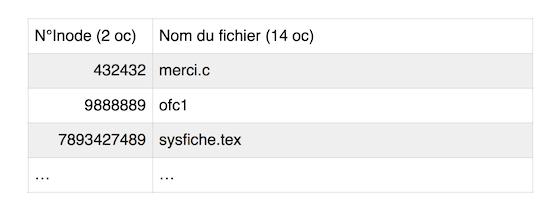
\includegraphics{rep_unix}
\\
\paragraph{Linux}
Sous Linux, c'est un peu plus compliqué:\\
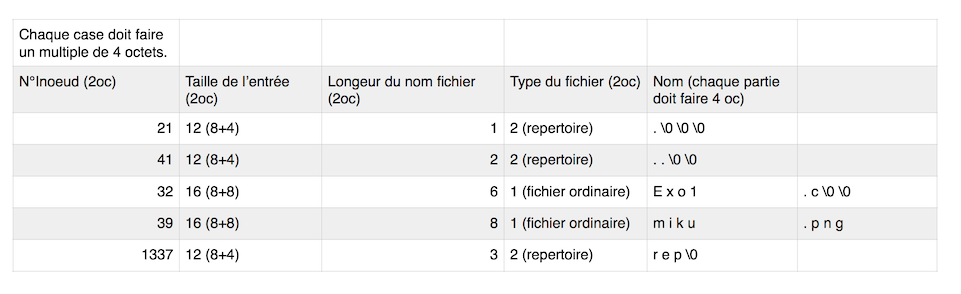
\includegraphics{rep_linux}
\\
La taille de l'entrée correspond à la somme des caractéristiques (8 octets) plus le nom du fichier. Vous devez vous demander à quoi correspondent les \emph{\textbackslash 0}; en fait, chaque case dans les noms de fichier doit faire \textbf{4 octets}; si on ne remplit pas la case, on ajoute des \textbackslash0. C'est tout.

\section{Manipulation des fichiers en C}
Parce oui, il faut bien jouer avec les fichiers en C.\\
Ce qu'il faut savoir, c'est que chaque processus possède une \emph{File Descriptor Table}, soit, en bon français, une \emph{Table de Descripteurs de fichiers}. En fait, un fichier est identifié au niveau système par un entier que l'on appelle \emph{file descriptor}. La table contient donc des descripteurs de fichiers qui pointent chacune sur un fichier.\\
Attention: les descripteurs 0, 1 et 2 sont réservés pour 3 fichiers très spéciaux, respectivement \emph{stdin}, \emph{stdout} et enfin \emph{stderr}. Cela veut aussi dire que \textbf{chaque programme} possède dans sa table de descripteur de fichier les descripteurs 0, 1 et 2.\\
Enfin, le système d'exploitation possède une table commune à tous les processus; c'est la \emph{Table des fichiers ouverts}. Cette table permet au système de savoir quel fichier est ouvert par qui et avec quels droits. On ne va pas s'étendre dessus, c'est pas très intéressant.
\paragraph{}
Sur U/L, il faut passer par plusieurs étapes afin d'utiliser un fichier dans un programme C: il faut \textbf{ouvrir} le fichier, faire son petit traitement (\textbf{lecture, écriture}, etc) puis \textbf{fermer} le fichier. Tout cela se fait par le biais d'appels systèmes que nous allons détailler.

\subsection{Ouvrir un fichier avec \emph{open( )}}
\emph{open( )} se présente de la manière suivante:
\begin{verbatim}
int open( const char *fichier, int flag );
\end{verbatim}
Commençons par les paramètres. \emph{*fichier} représente ici le nom du fichier \textbf{et son chemin}. Le \emph{flag} représente en fait une constante définie dans \emph{fcntl.h} qui définit les conditions dans lesquelles on souhaite ouvrir le fichier. Il en existe 4 d'importantes:
\begin{itemize}
\item{O\_RDONLY, comme Open\_ReadONLY, va ouvrir le fichier en lecture uniquement}
\item{O\_WRONLY, ouvre le fichier en écriture uniquement}
\item{O\_RDWR, ouvre le fichier en lecture et écriture}
\item{O\_APPEND, ouvre le fichier en écriture \textbf{en fin de fichier}}
\end{itemize}
Enfin, \emph{open( )} renvoie un entier (ou -1 si il se plante), qui correspond en fait au fameux \textbf{file descriptor}. Il est donc primordial de récupérer la valeur de retour d'open!
\paragraph{Exemple}
Imaginons que l'on souhaite ouvrir un fichier \emph{fic} se trouvant à \emph{/home/mooshi/rep} en lecture et écriture, sachant que l'on se trouve dans un autre répertoire que le fichier \emph{fic}; on doit écrire:
\begin{verbatim}
int fd = open("/home/mooshi/rep/fic", O_RDWR);
\end{verbatim}
Et \textsc{c'est gagné}.

\paragraph{Création d'un fichier} À noter: \emph{open()} permet aussi de créer un fichier, selon les flags que l'on met. Si on utilise \emph{O\_CREAT}, on doit rajouter un paramètre pour les droits. Regardez l'exemple, ça sera plus clair.
\begin{lstlisting}
/* Je souhaite créer un fichier oui avec des droits pour tout le monde */
int fd_oui = open("oui", O_CREAT, 0777);

/* Je souhaite créer un fichier merci avec des droits que pour moi
et seulement si il existe pas déjà */
int fd_merci = open("merci", O_CREAT | O_EXCL, 0700);
\end{lstlisting}
Le 3eme paramètre est un octal qui définit les droits. Vous vous rappelez de \emph{chmod}? C'est la même chose.

\subsection{Lire dans un fichier avec \emph{read( )}}
Regardons \emph{read( )}:
\begin{verbatim}
size_t read( int fd, void *buf, size_t nbOct )
\end{verbatim}
\textit{Mr.Toutlemonde}: omg c'est quoi ce size\_t??????? \\
\\
\emph{size\_t} correspond juste à un int. C'est juste pour montrer que ce int désigne une taille en octets.\\
Maintenant, regardons les paramètres. En premier, on retrouve notre cher \emph{file descriptor} que l'on a récupéré un peu plus tôt.\\
Pour le deuxième paramètre, il va falloir éclaircir la notion de \textbf{buffer}. Un buffer est une sorte de paquet d'une taille définie dans laquelle on va mettre des données. Très généralement, c'est un tableau de caractère qui occupe le rôle de buffer.\\
Enfin, le dernier paramètre correspond au nombre d'octets que l'on souhaite lire dans le fichier.\\
\emph{read( )} retourne le nombre d'octets effectivement lu dans le fichier.
\paragraph{Exemple}
Reprenons notre fichier fic du premier exemple. On souhaite lire son contenu sur 20 octets.
\begin{lstlisting}
char buf[20]; // On cree un buffer de taille 20 octets
int nbOctetsLus = read(fd, buf, 20); //On lit 20 octets du fichier
\end{lstlisting}
\textit{Mr.Toutlemonde}: ouais mais il va où le contenu du fichier???\\
Ben il va \sout{dans ton cul} ENFIN, non, mais on va voir ça tout de suite avec \emph{write}.

\subsection{Écrire dans un fichier avec \emph{write( )}}
En fait, les données lues vont dans notre buffer, c'est à dire, dans l'exemple précédent, \emph{buf}. \emph{write( )}, au lieu d'écrire dans le buffer depuis le fichier, va écrire dans le fichier depuis le buffer. Ainsi, on peut noter de nombreuses similitudes entre \emph{write( )} et \emph{open( )}:
\begin{verbatim}
size_t write(int fd, void *buf, size_t nbOct)
\end{verbatim}
Ici, nbOct représente le nombre d'octet que l'on souhaite écrire dans le fichier et cette primitive renvoie ici le nombre d'octets effectivement écrits dans le fichier.\\
Souvent, on fait travailler \emph{open} et \emph{write} à la suite, puisque on utilise plusieurs fois le buffer.
\paragraph{Exemple}
On reprend l'exemple du dessus. Maintenant qu'on a lu 20 octets dans notre buffer, on va essayer d'écrire dans un nouveau fichier.
\begin{lstlisting}
int newFic = open("fic2", O_CREAT, 0755); //On créé un nouveau fichier "fic2"
if (newFic != -1)
	int nbOctetsEcrits = write(newFic, buf, 20);
\end{lstlisting}
Voilà. On a écrit 20 octets dans un nouveau fichier fic2.

\subsection{Se déplacer dans un fichier avec \emph{lseek( )}}
Pas important. On verra plus tard.

\subsection{Fermer un fichier avec \emph{close( )}}
Là, c'est facile. \emph{close( )} ne prend qu'un paramètre, et c'est le \emph{file descriptor}.
\paragraph{Exemple}
Maintenant qu'on a écrit et lu nos fichiers fic et fic2, on les ferme.
\begin{lstlisting}
close(fd);
close(newFic);
\end{lstlisting}




\chapter{Pipes}
\epigraph{"Ça sent le pipeau ton histoire. Le pipeau !"}{Dave - La Classe Américaine}
Les processus (pour l'instant d'une même machine) peuvent communiquer entre eux par le biais de \emph{pipes}. Un pipe, c'est un tube par lequel on fait passer des informations. Un processus peut écrire et lire dans un pipe, cependant il n'y a \textbf{qu'un seul lecteur et qu'un seul écrivain par pipe}. Si on veut que deux programmes communiquent dans les deux sens, il faut créer deux pipes.
On va commencer par les \textbf{tubes anonymes}.\footnote{et on va faire que ça parce bon}

\section{Tubes anonymes}
\subsection{Créer un tube}
Afin de créer un tube, il faut utiliser l'appel système \emph{pipe( )}. Cet appel système prend en paramètre un tableau d'entier de taille 2. Regardez l'exemple:
\begin{verbatim}
int desc[2];
pipe(desc);
\end{verbatim}
Pourquoi un tableau d'entier de taille 2? Tout simplement car on aura dans ce tableau les \emph{file descriptor} qui correspondent à l'entrée du tube (ici \textbf{desc[1]}) et la sortie du tube (ici \textbf{desc[0]}). Bien sur, je pars du principe que vous savez ce que sont les \emph{file descriptor}, donc continuons.

\subsection{Écrire dans un tube}
Vous vous souvenez de \emph{write( )} qu'on utilisait pour écrire dans un fichier? C'est la même chose ici, sauf qu'on met le file descriptor de l'entrée du tube. On a donc:
\begin{verbatim}
char buffer[20]; // On a notre buffer de 20 octets
write(desc[1], buffer, 20); // On souhaite écrire dans notre pipe 20 octets de notre buffer
\end{verbatim}
Et voilà, c'est gagné.

\subsection{Lire depuis un tube}
Là encore, ça ressemble beaucoup à \emph{lire dans un fichier}:
\begin{verbatim}
char bufferLecture[20];
read(desc[0], bufferLecture, 20); //On veut lire 20 octets depuis le pipe dans notre buffer
\end{verbatim}

\subsection{Communiquer entre deux processus}
Le problème des tubes anonymes, c'est que les deux processus qui veulent communiquer doivent forcément connaitre les file descriptor. Ainsi, il faut que l'un des processus soit créé après la création du pipe. Par exemple:
\begin{lstlisting}
int main()
{
	int desc[2];
	pipe(desc);
	
	pid_t fils = fork();
	
	if(fils==0)
	{
		close(desc[0]);
		char bufferEcriture[]="un message pour mon papa";
		write(desc[1], bufferEcriture, strlen(bufferEcriture));
		exit(0);
	}
	
	wait(NULL);
	char bufferLecture[100];
	close(desc[1]);
	read(desc[0],bufferLecture,strlen(bufferEcriture));
	exit(0);
}
\end{lstlisting}
Il faut aussi s'assurer de \textbf{fermer} les extrémités - comprendre les \emph{desc[]} - inutilisés par chaque processus. Dans l'exemple ci-dessus, le fils n'est qu'un écrivain; par conséquent, on ferme l'extrémité de lecture - desc[0] -. De même pour le père, qui n'est que lecteur, on ferme d'abord l'extrémité d'écriture - desc[1] -.
Et voilà, on a bien établi une communication entre 2 processus!\\
On peut résumer tout ça en un schéma:\\
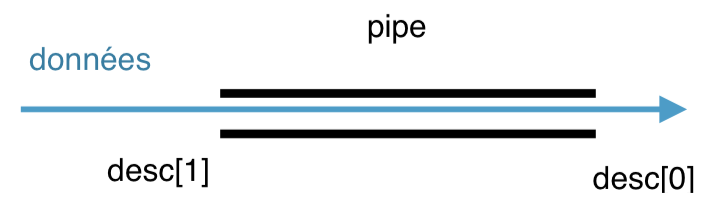
\includegraphics{pipe}

\section{Redirection de tubes aka \emph{dup2( )}}
Vous vous souvenez de \emph{dup2( )}? Vous savez, le cours ou vous avez \sout{rien} tout compris? Eh ben on va en reparler à travers un petit exercice:\footnote{inspiré de http://www.zeitoun.net/articles/communication-par-tuyau/start}\\
\textbf{Bouyou-Geauchamps}: \textit{Faites un programme qui execute l'équivalent de la commande "\emph{ls | wc}", sinon je \textbf{COLLOOOOOOOOOOOOO-}}\\

Comme vous êtes des gens vraiment \emph{too stongue}, vous avez certainement les étapes en tête:
\begin{itemize}
\item{Le processus père créé un processus fils, qui exécute \emph{ls}}
\item{La sortie standard du processus fils est \textbf{redirigée} vers l'entrée standard du père}
\item{Le père execute ensuite wc}
\item{\textit{C'est gagné}}
\end{itemize}

L'étape 1 est relativement facile:
\begin{lstlisting}
int main( int argc, char ** argv )
 {
   pid_t pidFils = fork();

   if (pidFils == 0)
     {
       execlp("ls", "ls", NULL);
       return 1;
     }

   wait(NULL);
   execlp("wc", "wc", NULL);
   return 2;
 }
\end{lstlisting}

La difficulté se passe évidemment sur la redirection. Il faut nécessairement créer un pipe qui fera la communication entre le père et le fils - on appellera ce pipe \emph{pipeCom} - mais pour la suite?\\
Comme vous l'avez deviné, il faut utiliser \emph{dup2( )}.\\
\emph{dup2( )} se présente de la manière suivante:
\begin{verbatim}
int dup2(int fdSource, int fdCible);
\end{verbatim}
En fait, \emph{dup2( )} permet de copier le file descriptor en deuxième argument dans le premier.

Dans notre exercice, cela se traduit donc par une \textbf{redirection} de la sortie standard du fils sur l'entrée du pipe \emph{pipeCom} et une redirection de la sortie du pipe \emph{pipeCom} sur l'entrée standard du père.\\ Regardez le schéma pour un peu plus de clarté:\\
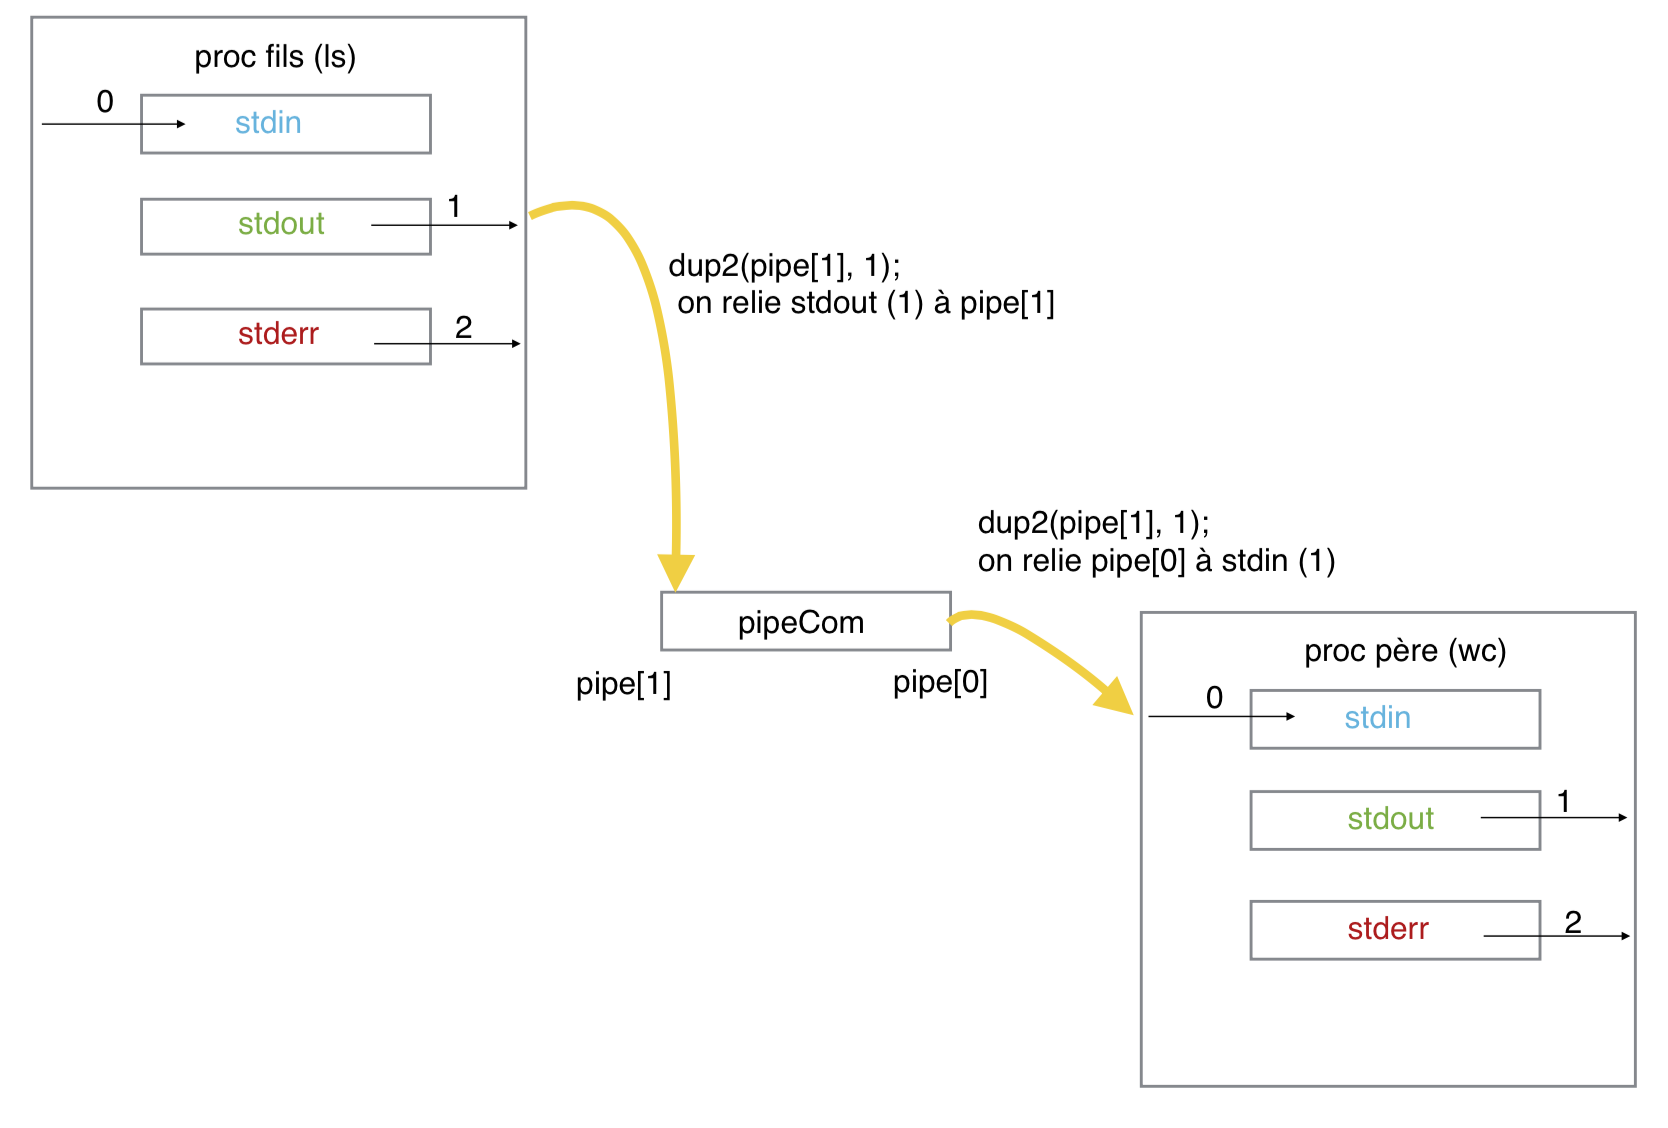
\includegraphics[scale=0.25]{dup2}
\\ Et maintenant, voilà notre code:
\begin{lstlisting}
int main( int argc, char ** argv )
 {
   pid_t pidFils = fork();
   int pipeCom[2];
   pipe(pipeCom);

   if (pidFils == 0)
     {
       close(pipeCom[0]);
       dup2(pipeCom[1],1);
       close(pipeCom[1]);
       execlp("ls", "ls", NULL);
       return 1;
     }

   wait(NULL);
   close(pipeCom[1]);
   dup2(pipeCom[0],0);
   close(pipeCom[0]);
   execlp("wc", "wc", NULL);
   return 2;
 }
\end{lstlisting}
On n'oublie pas de fermer les entrées/sorties inutiles pour éviter des embrouilles, et c'est gagné!




\chapter{Threads}
\epigraph{"Ça m'a l'air d'être un bordel..."}{La Classe Américaine}

\section{Préambule : Pointeurs et pointeurs de fonction}
\subsection{Pointeurs (lol S1)}
Faisons un petit rappel sur les pointeurs (get\_bellik):
\begin{itemize}
\item{Un pointeur se déclare sous la forme <type>* <nomDuPointeur>; il doit obligatoirement pointer sur une variable.}
\item{Un pointeur comporte l’adresse de la variable sur laquelle il pointe.}
\item{Afin d’accéder au contenu de la variable sur laquelle le pointeur pointe, il faut utiliser \emph{*<pointeur>}}.
\item{Utiliser <pointeur> permettra d’accéder à l’adresse de la variable pointée.}
\end{itemize}
En gros, un pointeur est une adresse, plus précisément celle de la variable pointée.

\subsection{Pointeurs de fonction}
Avant d'attaquer les threads, intéressons nous aux pointeurs de fonction.
Un pointeur de fonction est donc une variable qui désigne une fonction. Comme toute variable, on peut utiliser un pointeur de fonction en tant que variable dans une fonction, mais aussi et surtout comme un paramètre dans une fonction.\\
Un pointeur de fonction se déclare de la manière suivante:
\begin{verbatim}
void *pointeurFonction;
\end{verbatim}
Enfin, on peut créer directement des pointeurs de fonction avec un corps, tout comme une fonction "normale", sauf qu'on ajoute un \textbf{*} devant le nom de la fonction.
\begin{verbatim}
void *nomDeMaFonction([paramètres])
{
	/* corps de la fonction */
}
\end{verbatim}


\section{La notion de thread}
Vous vous souvenez des processus? Un programme englobe des processus, un processus englobe des threads. 
En fait, un thread est, \emph{une unité d'éxecution plus fine qu'un processus}; c'est pour cela qu'on appelle les threads des \emph{processus légers}.\\
Le but des threads est de pouvoir executer plusieurs parties d'un programme en parallèle. 
La différence majeure avec les processus est que les threads \textbf{partagent tout} entre eux. 
En effet, lorsque on créé un processus, le fait de modifier quelque chose dans le processus fils n'impactait pas le processus père. 
Avec les threads, ce n'est pas le cas. Par exemple, si un thread modifie une variable globale, cette variable sera modifiée pour \textbf{tous les threads}.
Il faut donc faire attention !
Enfin, notez que tous les threads dépendent du \textbf{thread principal}; si le thread principal se termine, tous les autres threads se terminent aussi.

Un thread s'identifie avec un pthread\_t. De la meme manière que la fonction \emph{getpid()}, il est possible d'obtenir l'identifiant d'un thread avec la fonction \emph{pthread\_self( )}.
\section{Création de thread et attente de terminaison}
Pour créer un thread, on utilise la fonction \emph{pthread\_create( )}. Cette fonction se présente de la manière suivante:
\begin{verbatim}
int pthread_create(pthread_t *thread, const pthread_attr_t *attr, void *(*fonc)(void*), void *arg);
\end{verbatim}
Regardons tranquillement les paramètres et leur rôle:
\begin{itemize}
\item{\emph{thread} représente un pointeur (ou une adresse) sur un objet de type \emph{pthread\_t} qui sera l'identifiant du thread après l'execution de cette fonction;}
\item{\emph{attr} représente le ou les attributs du thread, on peut voir ça comme les options de la fonction open();}
\item{\emph{fonc} représente un \textbf{pointeur de pointeur de fonction} - vous suivez? -. Ça sera la fonction exécutée par le thread.;}
\item{\emph{arg} représente un argument passé pour la fonction, il faut que ce soit un pointeur sans type (comprendre \emph{void *}), utiliser un cast si besoin. C'est donc le paramètre que va utiliser le thread pour la fonction donnée précédemment;}
\end{itemize}

Après avoir créé un thread, il faut bien le terminer. Il faut donc utiliser:
\begin{verbatim}
pthread_exit(void *valeurRetour);
\end{verbatim}
\emph{valeurRetour} est donc un pointeur non typé sur une valeur de retour. Concrètement, cela veut dire qu'il faut faire un cast sur l'adresse de la variable que l'on souhaite retourner.
Enfin, sachez que \emph{pthread\_exit()} ne tue pas réellement le processus. On verra d'autres manières de le faire dans la partie qui va suivre.

Tout cela parait très flou? Regardons alors un exemple.

\begin{lstlisting}
#include<pthread.h>

/* Voici la fonction qui sera exécutée par le thread. 
 *  Elle prend un paramètre int. */
void *fonction_thread(void *nombre)
{
    /* on récupère ici notre paramètre en faisant un cast.
        On cherche à récupérer le contenu d'un pointeur de type int */
    int nombreParam = *((*int) nombre);

   /* on affiche notre paramètre */
    printf("Le paramètre passé est %i \n", nombreParam);
    
    /* enfin, on termine le thread et on renvoie notre nombre.
    	Pour cela, il faut faire un cast sur l'adresse
	de la variable que l'on veut renvoyer */
    pthread_exit( (void*) &nombreRetour); 
}

int main(int argc, char **argv)
{
	pthread_t threadFils;
	int param = 5;
	
	/* on créé un thread qui execute fonction_thread 
	    on passe aussi un paramètre "param" */
	pthread_create(&threadFils, NULL, fonction_thread, (void*) &param); 

	/* on déclare un void* pour lire le retour */
	void *ret1;
	
	/* maintenant on attend la fin du thread
	   et on lit sa valeur de retour
	   On oublie pas de caster ret1 selon
	   le type de retour attendu */
	pthread_join(threadFils, (int*) ret1); 
	
	/* #cterminé */
	exit(0);
}
\end{lstlisting}	

\section{Autres manières d'arrêter un thread}
%Je suis un Thread qui veut arrêter son fils (ou un putain de random qui veux faire chier un autre thread), dans ce cas j'utilse la fonction\newline

\subsection{Arrêter un thread sans code de retour}
Dans certains cas, on peut libérer les ressources utilisées par un thread sans se soucier de son code de retour. Pour cela, on utilise:
\begin{verbatim}
pthread_detach(pthread_t thread_a_arreter);
\end{verbatim}
Cette fonction permet donc de tuer réellement un thread dés qu'il a fini réellement son travail, pas comme \emph{pthread\_exit( )}.

\subsection{Envoyer un signal pour tuer un thread (cancel)}
Tout comme les processus, il est possible de forcer l'arrêt d'un thread, mais aussi de bloquer le signal d'arrêt.
Pour arrêter un thread, il faut utiliser:
\begin{verbatim}
int pthread_cancel(pthread_t thread);
\end{verbatim}
avec \emph{thread} étant l'identifiant du thread que vous avez envie d'arrêter. \textbf{Cependant}, tout comme les processus et les signaux, un thread est capable de bloquer cette demande d'arrêt.

\subsection{Modification du comportement lors d'une demande de cancel}
Il existe deux fonctions permettant de modifier ce comportement:
\begin{verbatim}
int pthread_setcancelstate(int etat, int *etat_ancien);
\end{verbatim}
et
\begin{verbatim}
int pthread_setcaneltype(int mode, int *mode_ancien);
\end{verbatim}
Commençons par \emph{setcancelstate}.

\paragraph{pthread\_setcancelstate} permet de définir si le thread accepte ou pas les \emph{cancels}. On a donc que deux modes possibles:
\begin{itemize}
\item{\emph{PTHREAD\_CANCEL\_DISABLE} pour que le thread bloque tous les cancels;}
\item{\emph{PTHREAD\_CANCEL\_ENABLE} pour que le thread reçoive tous les cancels. C'est le mode par défaut.}
\end{itemize}

Un petit exemple pour la route:
\begin{verbatim}
/* je bloque tous les cancels */
pthread_setcancelstate(PTHREAD_CANCEL_DISABLE, NULL);
\end{verbatim}


\paragraph{pthread\_setcanceltype} permet de définir \textbf{comment} le thread accepte les \emph{cancels}. On a, là aussi, que deux modes possibles:
\begin{itemize}
\item{\emph{PTHREAD\_CANCEL\_ASYNCHRONOUS} pour que le thread traite les cancels à tous les instants;}
\item{\emph{PTHREAD\_CANCEL\_DEFERED} pour que le thread ne traite les cancels qu'a un certain moment. C'est le mode par défaut.}
\end{itemize}
Développons un peu cette histoire de \emph{CANCEL\_DEFERED}: en fait, cela veut dire que les cancels reçus par un thread ne seront traités qu'a l'exécution (par le thread) de certaines fonctions, qui sont \emph{pthread\_join( ), pthread\_testcancel( )} ou \emph{pthread\_cond\_wait}. Cela veut dire que les cancels reçus n'auront pas d'impact sur le thread jusqu'a que ce dernier exécute une des 3 fonctions citées auparavant.



\chapter{Programmation réseau en C}

\epigraph{"Avec le protocole \emph{TCP}, mes informations sont \textsc{complètes} et en \textsc{très bon état} ! \emph{Trékontan}"}{TG Biga, \textsc{brocantier}}

NB: Si vous avez le temps et l'envie, allez lire le \emph{Beej's Guide to Network Programming}, un guide très bien foutu à propos de tout ce bordel.

\section{Rappels et notions}
\subsection{Adresses ip \& ports}
Comme \textsc{Momo} nous l'a appris le semestre dernier, une communication réseau a besoin de connaître d'où elle vient et où elle va. On utilise donc des \emph{adresses ip} associé à un \emph{port}.\\
Il existe deux types d'adresses ip:
\begin{itemize}
\item{IPV4, qui est certainement le plus connu, et qui se présente par exemple de cette manière: 192.0.0.1;}
\item{IPV6, qui est assez nouveau, qui ressemble à ça: 2001:db8:0:85a3:0:0:ac1f:8001} 
\end{itemize}
Ne vous inquiétez pas; dans le contexte actuel, on ne se concentra que sur les adresses \emph{IPV4}.

Quant au port, il se présente sous la forme d'une série de chiffres qui permettent de \emph{préciser} là où doit aller l'information. Chaque port est dédié à un programme, afin d'éviter de mélanger les informations dédiés par exemple à la messagerie à celle dédié à un jeu vidéo en ligne par exemple. Sachez que les ports ayant un numéro inférieur à \emph{1024} sont considérés comme spéciaux, ainsi, ne prenez pas un port ayant un numéro inférieur à 1024.

\subsection{Protocoles UDP \& TCP}
Pour communiquer sur le réseau, il existe deux protocoles de communication: \emph{UDP} et \emph{TCP}.
\paragraph{UDP}
signifie \emph{User Datagram Protocol}. En gros, l'UDP permet d'envoyer très rapidement des informations, et pour cause: on \textbf{ne vérifie pas} si l'information est bien arrivée. C'est aussi pour cela que l'UDP est ce qu'on appelle un protocole \emph{connectionless}: on a pas à faire de \emph{connexion préalable} avant d'envoyer l'information. On met une adresse, on envoie l'information, \textsc{et c tou}. Pour faire un parallèle avec la vraie vie, voyez l'\emph{UDP} comme \textit{une lettre postale}: on envoie l'information, on sait pas si le destinataire existe, mais on s'en fout puisque on a déjà envoyé l'information.

\paragraph{TCP} signifie \emph{Transmission Control Protocol}. Contrairement à l'\emph{UDP}, il faut d'abord établir une communication avec l'écouteur avant d'envoyer des informations. Comme son nom l'indique, il y a un \emph{contrôle} des informations, ainsi on est assuré d'envoyer les informations dans le \emph{bon ordre} mais aussi de façon \emph{complète}. Comme le dit \textsc{Bouyou}, on peut comparer le protocole \emph{TCP} à \emph{une conversation téléphonique}. Le désavantage du protocole \emph{TCP} par rapport à l'\emph{UDP} est sa vitesse, mis à part ça...


\subsection{Sockets}
Les \emph{sockets} sont l'intermédiaire entre une application et la couche réseau du système. Tout comme \emph{tout et n'importe quoi} dans \textsc{Unix}, les \emph{sockets} sont aussi des fichiers ! Ainsi, les sockets sont identifiés avec un \emph{file descriptor}, eh oui. Par conséquent, il existe moults appels systèmes permettant d'utiliser ces sockets.\\
Mais, ne vous inquiétez pas, nous reviendrons sur leur utilisation plus tard; pour l'instant, regardons les différents types de \emph{sockets} disponibles. 

On a à notre disposition 2 types de sockets\footnote{il existe un 3è type, que l'on appelle "raw", mais ici on ne les utilisera pas}: chacune correspondant à un protocole.
\begin{itemize}
\item{les \emph{Stream Sockets}, donc \emph{socquettes de flux} en bon Francais, utilisent le protocole \emph{TCP}. Ils ont donc un très bon niveau de qualité de transmission de données, et on est assuré d'avoir l'info dans le bon ordre et en bon état;}
\item{les \emph{Datagram Sockets}, donc \emph{sockets de pacquets}, utilisent le protocole \emph{UDP}. Allez voir en haut si vous voulez une description de l'udp.}
\end{itemize}

\subsection{Structures en C}
Petit rappel de C: une structure est une sorte d'objet, mais en C. Une structure se déclare de la façon suivante:
\begin{lstlisting}
typedef struct{
	/* random attributs */
	int a;
} nomDeLaStructure;
\end{lstlisting}
On peut ensuite l'utiliser et accéder aux attributs comme ça:
\begin{lstlisting}
nomDeLaStructure bruno = {a=1};
/* affiche 1 */
printf("%i", bruno.a);
bruno.a = 2;
/*affiche 2*/
printf("%i", bruno.a);
\end{lstlisting}
Retenez aussi que pour accéder à un attribut d'un pointeur, on utilise la notation \emph{->}.


\section{Établir une connexion en UDP, partie Client} 
Pour établir une connexion, c'est très simple: il suffit de respecter un certain nombre d'étapes à la lettre. On va commencer par le plus simple, l'UDP.
\subsection{Créer un socket et préparation de la connexion}
Avant toute chose, le client doit savoir \textbf{où} se connecter. Cela veut donc dire que le client doit connaître au préalable le nom de l'hôte et le port sur lequel il va se connecter.\\
Ensuite, on créé un socket avec ces informations et on se prépare à envoyer nos informations en modifiant ce socket. En C, cela se représente de la manière suivante:
\begin{lstlisting}
#define PORT 1337

int main(int argc , char ∗∗argv){

	/* Préparation de notre socket + sockaddr */
	int socket_fd;
	/* Ce sockaddr sert a contenir les informations du serveur */
	struct sockaddr_in sockServer = {0};
	/* Ce pointeur pointera vers une structure
	   qui contiendra les informations correspondant
	    à l'hote que l'on souhaite contacter */
	struct hostent *h;
	
	/* On remplit notre pointeur de structure avec
	    l'information trouvée par gethostbyname */
	h=gethostbyname(argv[1]);
	/* On prépare notre socket */
	socket_fd = socket(AF_INET, SOCK_DGRAM, 0);
	
	/* On remplit enfin notre sockServer
	   On utilisera ce sockServer pour se connecter */
	sockServer.sin_family = AF_INET;
	sockServer.sin_port = htons(PORT);
	sockServer.sin_addr = *((struct in_addr *)h -> h_addr);
}
\end{lstlisting}

\subsection{Envoi/reception de message}
Maintenant qu'on a préparé notre connexion, on peut enfin utiliser notre \textsc{bon vieux} socket et sockAddr.\\
N'oubliez pas; vu qu'UDP est un protocole \emph{non connecté}, on a donc pas de connect, mais juste \emph{sendto} et \emph{recvfrom}.\\
Concrétement, on  a donc ça:
\begin{lstlisting}
/* Tout ce code se place à la suite du code mis en haut */
	/* on cherche à envoyer ce message */
	char message[] = "coucou";
	/* On envoie donc ce message par le biais du socket socket_fd
	   à travers le sockaddr sockServer, qu'on oublie pas de caster en sockaddr* */
	int sent = sendto(socket_fd , message, strlen(message), 0, (const struct sockaddr ∗)&sockServer , sizeof(struct sockaddr));

	/* On attend ensuite un message de la part du serveur
	    On prépare d'abord à recevoir les informations du serveur */
	struct sockaddr_storage sender;
	socklen_t addr_len = sizeof(sender); 
	memset(&sender , 0 , sizeof (sender));
	
	/* On va recevoir le message du serveur dans un char[] */
	char buffer[50];
	/* On attend donc le message du serveur par le biais du socket_fd */
	int rec = recvfrom ( socket_fd , buffer , sizeof (buffer) , 0 , (struct sockaddr∗)&sender , &addr_len );
/* Après, on peut faire ce qu'on veut du message qui se trouve dans le buffer */
	close(socket_fd);
	return(0);
}
\end{lstlisting}
Voilà, c'est tout pour la partie client. On va maintenant s'interesser à la partie serveur en UDP.

\section{Connexion en UDP, partie Serveur}
Le principe est à peu près le même que le client, à la différence que le serveur doit se bind sur un port défini, et qu'il doit d'abord attendre de recevoir un message avant d'en envoyer un.
Vu que j'ai pas envie de me faire chier, je vais reprendre le code du TP7, commenté:
\begin{lstlisting}
#define PORT 1337

/* Structure d'un abonne, rien de fabuleux */
typedef struct
{
	char nom[20];
	char numero[50];
} abonne;

int main(int argc, char **argv)
{
	/* Notre fabuleuse table d'abonnés */
	abonne tableAbonne[10] = {{ "Ouam","01 02 03 04 05" }, { "BruneOuais", "06 06 07 01 02" }, 
				  { "Steeve", "36 15 13 37 42 " }, { "Eli Assez", "06 69 69 69 69" },
				  { "Mozart", "01 01 01 02 02" }, { "Stravinsky", "01 99 99 13 37" }};

	/* Là aussi, on prépare nos informations */
	int sock_fd;
	/* Cette structure permet de préparer NOS informations */
	struct sockaddr_in socketServeur;
	
	/* On créé un socket */
	sock_fd = socket(AF_INET, SOCK_DGRAM, 0);
	
	/* On regle nos parametres */
	socketServeur.sin_family = AF_INET;
	socketServeur.sin_port = htons(PORT);
	socketServeur.sin_addr.s_addr = htonl(INADDR_ANY);
	
	/* On assigne notre sockServeur au socket créé */
	bind(sock_fd, (struct sockaddr *)&socketServeur, sizeof(socketServeur));

	/* On se prépare à recevoir le message et les informations du client */
	struct sockaddr_in socketClient;
	socklen_t addr_len;
	addr_len = sizeof socketClient;
	char buf[100];

	/* Notre serveur tourne en continu */	
	while(1) 
    {
	  	memset(&buf, 0, sizeof(buf));

		/* On lit le message du client */
		int read = recvfrom(sock_fd, buf, 100-1 , 0, 
				   (struct sockaddr *)&socketClient, &addr_len);
	
		/* Traitement du message */
		char abonne[50];
		strcpy(abonne,buf);
		abonne[read] = '\0';
		int i=0;
		int ret=1;
		while( ret != 0 && i<10 )
		{
			ret = strcmp(tableAbonne[i].nom, abonne);
			i+=1;
		}	
		char messRetour[50];
		if(ret == 0)
		{
			sprintf(messRetour,"Le numero de l'abonne est ");
			strcat(messRetour,tableAbonne[i-1].numero) ;
		}
		else
			sprintf(messRetour,"abonne inconnu");

		/* On envoie enfin le message au client */
		int sent = sendto(sock_fd, messRetour, strlen(messRetour), 
				  0, (struct sockaddr *)&socketClient, addr_len);
	}
	exit(0);
}
\end{lstlisting}
Pour résumer :
\begin{itemize}
\item{On prépare ses informations sur son sockAddr}
\item{On créé un socket d'écoute}
\item{On assigne notre sockAddr à ce socket avec \emph{bind()}}
\item{On lit depuis ce socket (\emph{recvfrom()}), on stocke les informations du client}
\item{On écrit sur ce socket (\emph{sendto()}) avec les informations du client}
\end{itemize}

\section{Connexion en TCP, partie client}
Là aussi, je vais commenter le code parce que.
\begin{lstlisting}
#define PORTS 6500

int main(int argc, char** argv)
{
	struct hostent *h;
	struct sockaddr_in sockClient;
	struct sockaddr_in sockServer;
	int sock;
	
	/* on créé un socket */
	sock = socket(AF_INET, SOCK_STREAM, IPPROTO_TCP);
	
	/* préparation de l'adresse locale */
	sockClient.sin_family = AF_INET;  //ipv4
	sockClient.sin_port = htonl(argv[2]); //dans ce programme on passe le port en parametre
	sockClient.sin_addr.s_addr = INADDR_ANY; //cela permet d'avoir une adresse automatique
	
	// On assigne notre sockaddr au socket
	bind(sock, struct sockaddr *)&sockClient, sizeof(sockClient);
	
	// on obtient les informations de l'hote distant
	h = gethostbyname(argv[1]);
	
	//On définit les parametres de l'hote
	sockServer.sin_family = AF_INET; //ipv4
	bcopy(h->h_addr, &sockServer.sin_addr, h->h_length); //on copie l'adresse trouvée en résultat dans le sockAddr serveur
	sockServer.sin_port = htons(PORTS);
	
	//On lance la connexion au serveur
	connect(sock, (const struct sockaddr *)&sockServer, sizeof(sockServer));
	
	char abonne[50];
	printf("Donnez un nom d'abonne");
	scanf("%s",abonne);
	
	/* On envoie des requetes tant qu'on a pas fait ctrl+d */
	while(!feof(stdin))
	{
		// On écrit sur le socket le message
		write(sock, abonne, strlen(abonne)+1);
		
		char telephone[12];
		// On lit depuis le socket le message du serveur
		read(sock,telephone,12);
		printf("%s \n saisir autre abonne", telephone);
		scanf("%s",abonne);
	}
	// Quand on a fini, on ferme le socket.
	close(sock);
	exit(0);
}
\end{lstlisting}
Résumons.
\begin{itemize}
\item{On prépare ses informations sur son sockAddr et celles du serveur}
\item{On créé un socket}
\item{On assigne notre sockAddr à ce socket avec \emph{bind()}}
\item{On obtient les informations sur l'hote avec \emph{gethostbyname( )}
\item{On copie l'adresse trouvée par \emph{gethostbyname( )} dans le sockAddr du serveur}
\item{On se connect avec notre socket au sockAddr du serveur}
\item{On lit et on écrit sur notre socket}}
\end{itemize}
Relativement facile non? Passons au serveur, ça va \emph{un peu} se corser.

\section{Connexion en TCP, partie Serveur}
Ce programme est relativement complexe car \textsc{Bouyou} a décidé de le rendre compliqué. Il s'agit en fait de bien faire la différence entre ce qui est important pour la connexion en TCP et ce qui était important pour le TD6.
\begin{lstlisting}
#define PORTS 6500

//Structure d'un abonné + tableau d'abonnés
struct abonne{
	char nom[30];
	char telephone[12];
} annuaire[] = {
	"bla", "01010101"
};

char msg[] = "erreur !";
void *service(void *);

int main(){
	int lg, sock, newsock, *ptint;
	struct sockaddr_in sockServeur;
	struct sockaddr_in sockClient;
	pthread_t pth_id;
	
	/* Création du socket d'écoute */
	sock = socket(AF_INET, SOCK_STREAM, IPPROTO_TCP);
	
	/* Préparation de l'adresse locale */
	sockServeur.sin_family = AF_INET; //ipv4
	sockServeur.sin_port = htons(PORTS); //sur le port défini en constante
	sockServeur.sin_addr.s_addr = htonl(INADDR_ANY); //on se bind sur n'importe quelle adresse
	
	/* On associe le socket à notre sockAddr */
	bind(sock, (struct sockaddr *)&sockServer, sizeof(sockServer));
	
	/* Dimensionnement de la file d'attente */
	listen(sockClient,30);
	
	/* Tant que le serveur tourne */
	while(1)
	{
		/* accept retourne un descripteur de socket pour chacune des connexions faites sur le socket sock */
		newsock = accept(sock, (struct sockaddr*)&sockClient, &lg);
		
		/* ne faites pas vraiment attention au reste, on cherche en fait à passer notre nouveau descripteur de socket à notre fonction de thread */
		ptint=(int) malloc(sizeof(int));
		*ptint = newsock;
		pthread_create(&pt_id, NULL, service, (void *)ptint);
		pthread_detach(pth_id);
	}
}

void *service(void * sockservice)
{
	int nb, l, j, i, test;
	char line[30];
	
	/* On met dans line le message écrit par le client */
	nb=read(*(int*)sockservice, line, 30);
	
	/* Ce n'est pas important pour le TCP, c'est juste du traitement */
	while(nb!=0)
	{
		l = strlen(line);
		for(j=0;j<l;j++)
			line[j] = (char) tolower((int)line[j]);
		i=test=0;
		while ((test==0) && (i<10))
		{
			if(strcmp(line,annuaire[i].nom) == 0)
				test=1;
			i++;
		}
		
		/* LÀ c'est important: on écrit sur le socketClient le message */
		if (test==1)
			write(*(int*)sockservice, annuaire[i-1].telephone,strlen(annuaire[i-1].telephone)+1);
		else
			write(*(int*)sockservice, msg, strlen(msg)+1);
		nb=read(*(int*)sockservice,line,30);
	}
	
	/* Une fois que c'est fini, on ferme le socket */
	close(*(int*)sockservice);
	pthread_exit(NULL);
}
\end{lstlisting}
Pour résumer simplement comment ça fonctionne coté serveur:
\begin{itemize}
\item{On prépare ses informations sur son sockAddr}
\item{On créé un socket d'écoute}
\item{On assigne un sockAddr à un socket avec \emph{bind()}}
\item{On écoute (\emph{listen( )}) puis on accepte (\emph{accept( )}) les connexions sur ce socket}
\item{On lit et on écrit depuis le socket retourné par \emph{accept( )}}
\end{itemize}


\chapter{Bonus et \sout{Taunts}}
Si vous voulez vraiment en savoir plus, lisez le \textsc{Beej's Guide to Network Programming}.\\
La programmation réseau en C utilise un tas de nouvelles structures et types qui peuvent sembler bizarres au premier coup d'oeil. Même si c'est pas obligatoire pour réussir les exercices, explicitons les structures utilisées.\\
\subsection{\emph{addrinfo} et \emph{getaddrinfo( )}}

\emph{addrinfo} se présente de la manière suivante:
\begin{lstlisting}
struct addrinfo {
    int              ai_flags;     // AI_PASSIVE, AI_CANONNAME, etc.
    int              ai_family;    // AF_INET, AF_INET6, AF_UNSPEC
    int              ai_socktype;  // SOCK_STREAM, SOCK_DGRAM
    int              ai_protocol;  // use 0 for "any"
    size_t           ai_addrlen;   // size of ai_addr in bytes
    struct sockaddr *ai_addr;      // struct sockaddr_in or _in6
    char            *ai_canonname; // full canonical hostname
    struct addrinfo *ai_next;      // linked list, next node
};
\end{lstlisting}
"Oula oula", allez vous me dire, "c'est quoi ce bordel monstre????"\\
\emph{addrinfo} est en fait une structure très importante, puisque elle va regrouper la majorité des informations permettant de créer un socket.\\
En fait, afin de savoir où se connecter, il faut appeler la procédure \emph{getaddrinfo( )}, qui remplira une structure \emph{addrinfo}.\\
Mais trève de blabla, regardons maintenant ses attributs:
\begin{itemize}
\item{\emph{ai\_family} indique le protocole ip desiré par les adresses ip renvoyées. On a soit \emph{AF\_INET} (protocole ipv4), \emph{AF\_INET6} (ipv6) ou \emph{AF\_UNSPEC} (les deux).
Dans notre cas, on utilsera \emph{AF\_INET};}
\item{\emph{ai\_socktype} indique le type de socket utilisé. Allez voir en haut pour avoir une description de ces sockets.}
\item{\emph{ai\_protocol} indique le protocole utilisé par les sockets. Mettez 0, cela suffira.}
\item{\emph{ai\_flags} indique des modifieurs. \emph{AI\_PASSIVE}, par exemple, permettera de remplir le \emph{sockaddr} automatiquement avec l'adresse de l'hôte. Très pratique pour faire un serveur!}
\end{itemize}

Maintenant, regardons \emph{getaddrinfo( )}:
\begin{lstlisting}
int getaddrinfo(const char *node,     // Adresse ip de l'hôte ou adresse http
                const char *service,  // Numero de port ou "http"
                const struct addrinfo *hints, // pointeur vers une structure 
                				//"addrinfo" préremplie
                struct addrinfo **res); //pointeur vers un pointeur d'addrinfo 
                			//(le resultat)
\end{lstlisting}
En fait, avant d'appeller \emph{getaddrinfo}, il faut créer une structure \emph{addrinfo} et un \emph{pointeur de structure addrinfo}.\\
La structure permettra de définir ce que l'on souhaite récupérer et le pointeur permettra de récupérer les \emph{addrinfo} correspondants à nos critères définis dans la structure.
\paragraph{En pratique} cela se présente de la manière suivante:
\begin{lstlisting}
struct addrinfo hints;
struct addrinfo *servinfo;
/* on initialise la structure */
memset(&hints, 0, sizeof hints);
/* on souhaite une connexion avec ipv4 et en UDP */
hints.ai_family = AF_INET;
hints.ai_socktype = SOCK_DGRAM;
/* on souhaite obtenir des infos pour se connecter à "127.0.0.1"
 * au port 1337 */
getaddrinfo(127.0.0.1, 1337, &hints, &servinfo);
/* maintenant, les résultats sont pointés par servinfo */
\end{lstlisting}
Maintenant, interessons nous à \emph{sockaddr}, structure qui possède des informations sur le socket.

\subsection{\emph{sockaddr}}
En réalité, il existe 3 types de \emph{sockaddr}:
\begin{itemize}
\item{\emph{sockaddr\_in}, qui contient des informations relatives au socket selon le protocole IPV4}
\item{\emph{sockaddr\_in6}, qui contient des informations selon le protocole IPV6}
\item{\emph{sockaddr}, qui est plus général que ses variantes \_in et \_in6. Dans les faits, on castera sockaddr\_in en sockaddr pour pouvoir utiliser \emph{connect}}
\end{itemize}
En plus de ces 3 types de sockaddr, il existe un dernier type de sockaddr, \emph{sockaddr\_storage}, qui permet en fait de stocker les informations du l'expéditeur. Je sais que tout cela semble très flou pour le moment, mais tout devrait s'éclaircir par la suite.\\
Pour le plaisir, voilà le contenu de la structure \emph{sockaddr} et \emph{sockaddr\_in}:
\begin{lstlisting}
struct sockaddr {
    unsigned short    sa_family;    // address family, AF_xxx
    char              sa_data[14];  // 14 bytes of protocol address
};

struct sockaddr_in {
    short int          sin_family;  // Address family, AF_INET
    unsigned short int sin_port;    // Port number
    struct in_addr     sin_addr;    // Internet address
    unsigned char      sin_zero[8]; // Same size as struct sockaddr
};

struct in_addr {
    uint32_t s_addr; // that's a 32-bit int (4 bytes)
};
\end{lstlisting}

\subsection{\emph{socket( )}}
\begin{verbatim}
socket(int domain, int type, int protocol)
\end{verbatim}
\emph{socket( )} retourne donc un int, qui correspond au fait à un descripteur de fichier. Il est donc primordial de récuperer la valeur de retour de socket.\\
Cet appel système prend donc 3 paramètres:
\begin{itemize}
\item{\emph{domain} correspond à la portée du socket. \textbf{AF\_UNIX} pour une portée locale, \textbf{AF\_INET} pour une communication par réseau.}
\item{\emph{type} correspond au type de socket utilisé. \textbf{SOCK\_DGRAM} pour une communication non connectée (udp), \textbf{SOCK\_STREAM} pour une connectée (tcp). On peut aussi mettre \textbf{SOCK\_RAW}, mais on ne l'utilisera pas ici.}
\item{\emph{protocol}, pas besoin de le présenter. \textbf{IPPROTO\_UDP} ou \textbf{IPPROTO\_TCP}. Laissez \textbf{0} et le système se débrouillera comme un grand.}
\end{itemize}

\subsection{\emph{bind( )}}
\begin{verbatim}
int bind(int sockfd, const struct sockaddr *addr, socklen_t addrlen);
\end{verbatim}
\emph{bind( )} permet d'attacher un socket - représenté par un descripteur de fichier - à une adresse réseau, c'est à dire un sockaddr.

\begin{itemize}
\item{sockfd, le descripteur d'un socket.}
\item{addr : un pointeur sur une structure de type sockaddr.} 
\item{addrlen : la taille en octets de la structure addr.}
\end{itemize}
Aujourd'hui, il est assez simple d'attacher une structure réseau, puisque c'est \emph{getaddrinfo( )} qui remplit une structure. Du coup, il est facile d'utiliser bind, puisque tout est déjà dans la structure pointée par res:
\begin{lstlisting}
/* Exemple tiré du TP7, coté serveur
 * on suppose qu'on a déjà déclaré nos structures */
getaddrinfo(NULL, SERVERPORT, &hints, &servinfo);
int socket_fd = socket(servinfo->ai_family, servinfo->ai_socktype, servinfo->ai_protocol);
bind(socket_fd,servinfo->ai_addr, servinfo->ai_addrlen);
\end{lstlisting}

\subsection{\emph{connect( )}}
\emph{connect( )} se présente de la manière suivante;
\begin{lstlisting}
int connect(int sockfd, struct sockaddr *serv_addr, int addrlen);
\end{lstlisting}

\end{document} 